\documentclass[11pt]{article}

\usepackage{xcolor}
\usepackage{fontenc}
\usepackage{enumitem}
\usepackage{multicol}
\usepackage{multirow}
% \usepackage{subfigure}
\usepackage{subcaption}
\usepackage{graphicx}
\usepackage[colorlinks=true]{hyperref}
\usepackage[margin=1in]{geometry}
\usepackage[style=numeric, backend=biber]{biblatex}
\addbibresource{solar_system.bib}
\usepackage{amsmath}
\usepackage{amsthm}
\newtheorem{proposition}{Proposition}
\usepackage{authblk}
\newcommand{\be}{\begin{equation}}
\newcommand{\ee}{\end{equation}}

\begin{document}
\title{\textsc{The Solar System}}
\author[1]{Johannes Kepler}
\affil[1]{
Imperial Mathematician, Prague}
\maketitle

\tableofcontents
\newpage

\section{Our Planetary Neighborhood}
\subsection{The Sun and Its Planets}
The Sun and its gravity-bound bodies form the Solar System \cite{kepler1609}. See \href{https://science.nasa.gov/solar-system/}{NASA
Solar System Exploration}. In increasing distance, the planets are

\begin{quote}
    Mercury, Venus, Earth, Mars, Jupiter, Saturn, Uranus, Neptune.
\end{quote}
The planets form two groups:
\begin{enumerate}[label=(\Roman*)]
    \item Inner planets
    \begin{itemize}[label=$\dagger$]
        \item Mercury, Venus, Earth, and Mars belong to this group.
        \item They are comparatively small and have solid surfaces.
        \item They are also called the terrestrial planets.
    \end{itemize}
    \item Outer planets
    \begin{itemize}[label=$\dagger$]
        \item Jupiter and Saturn are gas giants.
        \item Uranus and Neptune are commonly called ice giants
        \item All four outer planets possess ring systems.
    \end{itemize}
\end{enumerate}

\textcolor{blue}{The inner planets are small, dense, and relatively close to the Sun, } whereas \textcolor{red}{the outer planets are much larger and travel along considerably wider orbits}




\subsection{Portraits of the Solar System}
Figure \ref{fig:solar} shows the Sun and eight planets.\footnote{Sizes and distances are schematic.}
Compare Mars in Figure 1e with Jupiter in Figure \ref{fig:jupiter}.

\begin{figure}[t]
    \centering
    \textbf{Star}\\
    \vspace{0.5cm}
    \begin{subfigure}{0.3\textwidth}
        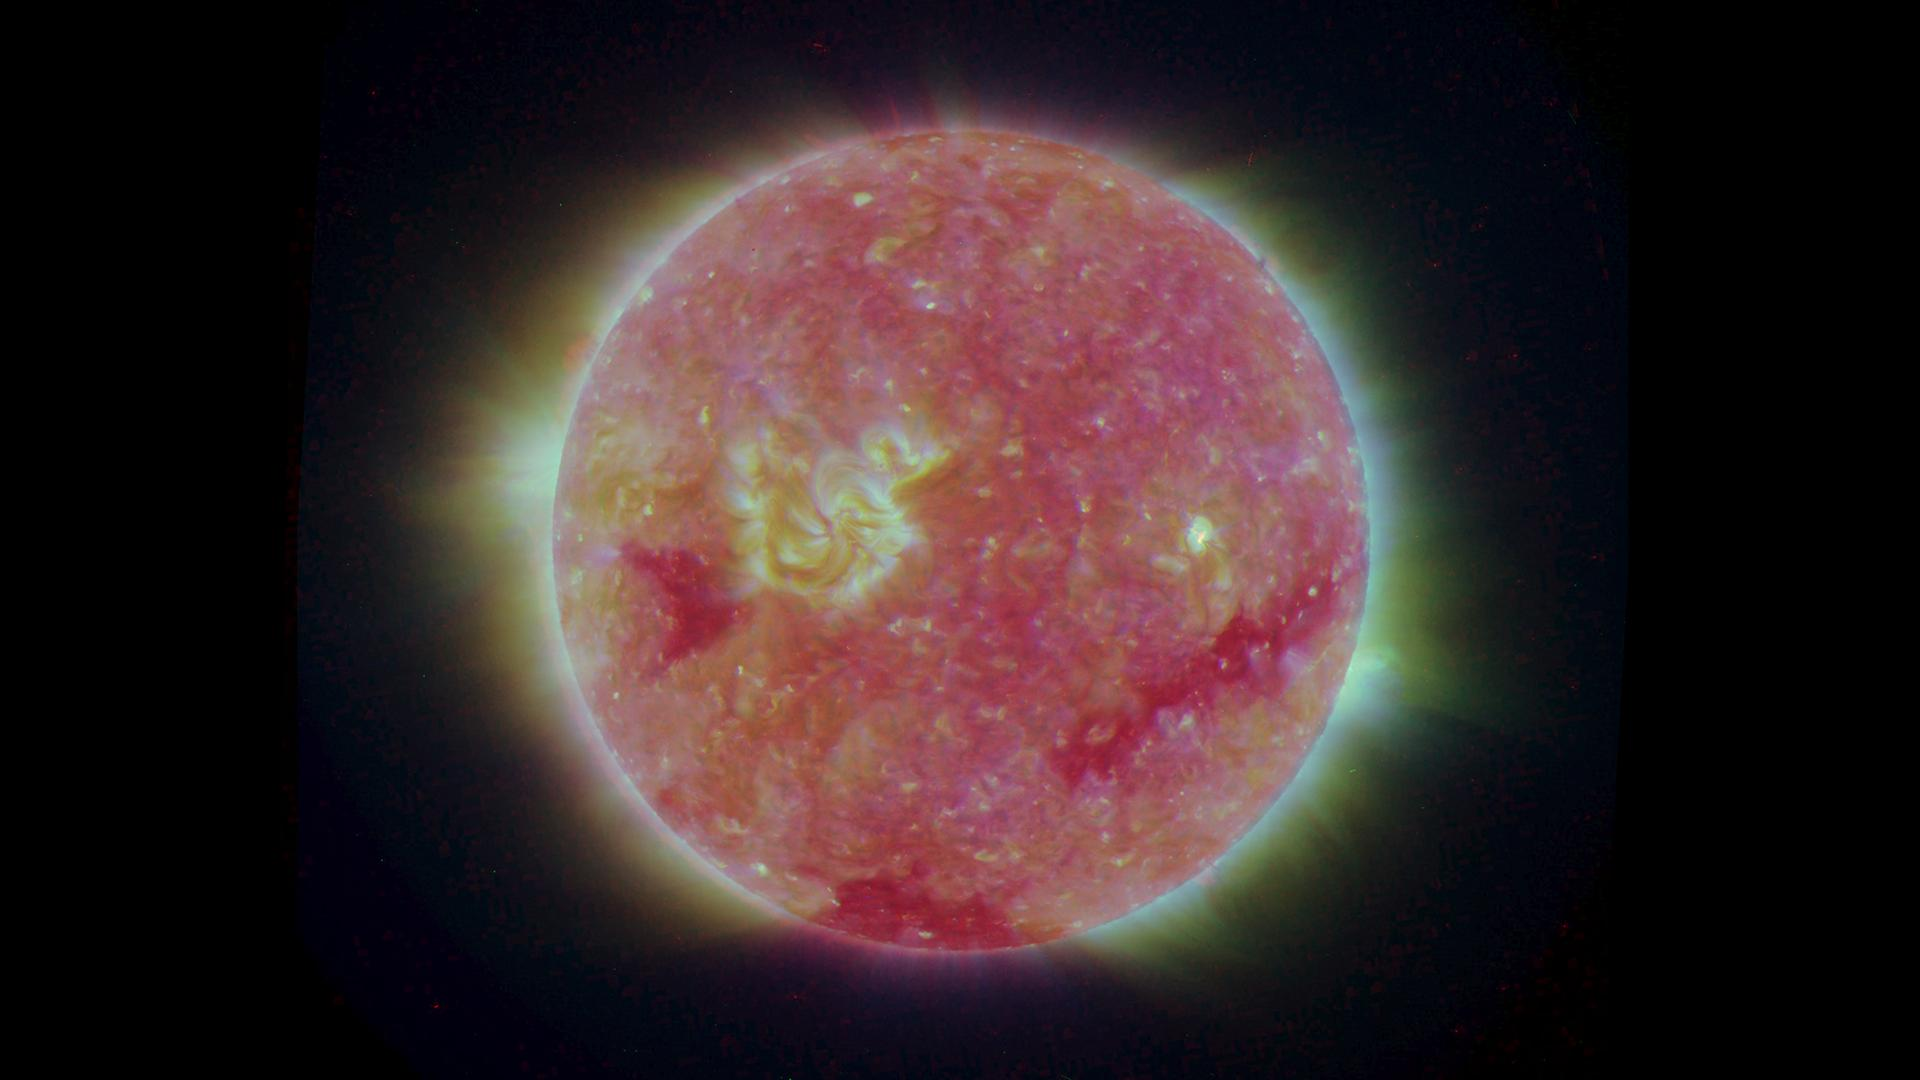
\includegraphics[width=\linewidth]{sun.png}
        \caption{The Sun}
    \end{subfigure}

    \vspace{0.5cm}
    \textbf{Inner Planets}\\
    \vspace{0.5cm}
    \begin{subfigure}{0.2\textwidth}
        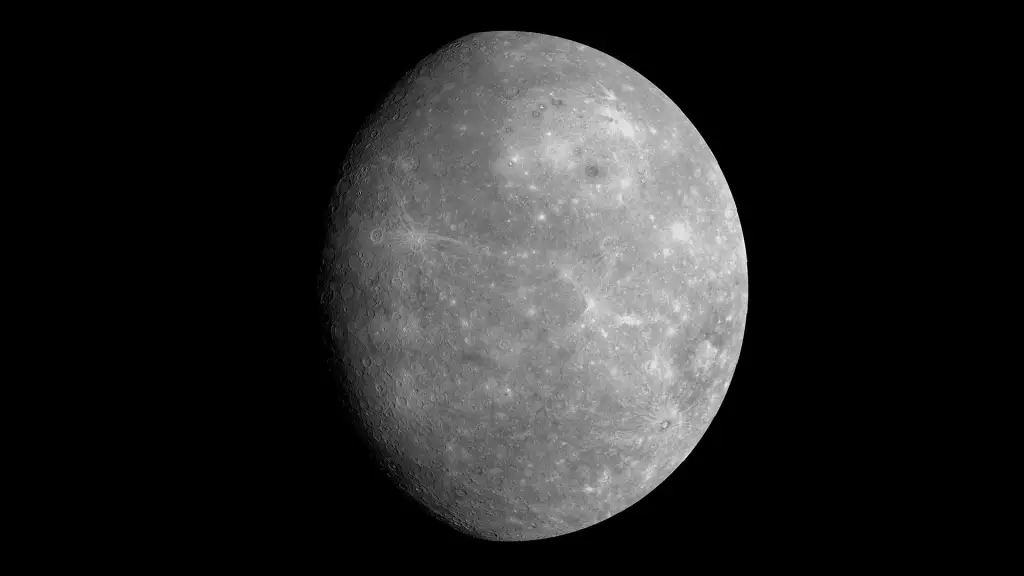
\includegraphics[width=\linewidth]{mercury.png}
        \caption{mercury}
        \label{fig:mercury}
    \end{subfigure}
    \hfill
    \begin{subfigure}{0.2\textwidth}
        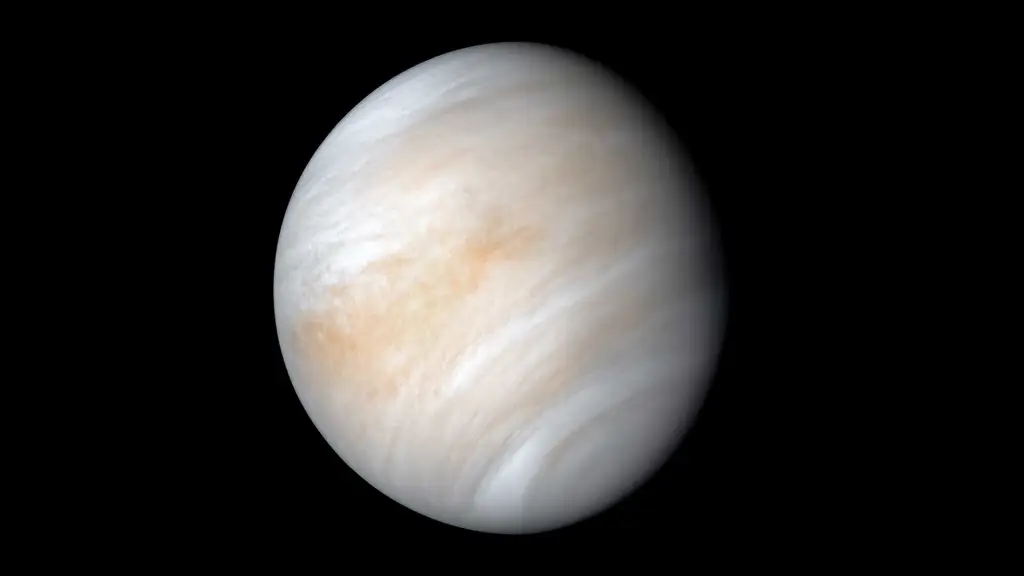
\includegraphics[width=\linewidth]{venus.png}
        \caption{venus}
        \label{fig:venus}
    \end{subfigure}
    \hfill
    \begin{subfigure}{0.2\textwidth}
        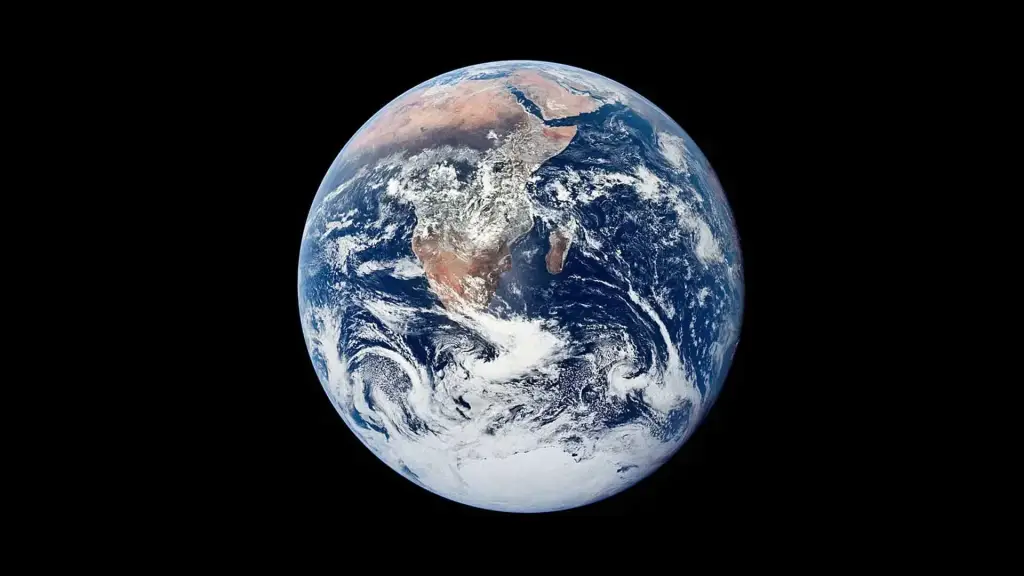
\includegraphics[width=\linewidth]{earth.png}
        \caption{Earth}
        \label{fig:earth}
    \end{subfigure}
    \hfill
    \begin{subfigure}{0.2\textwidth}
        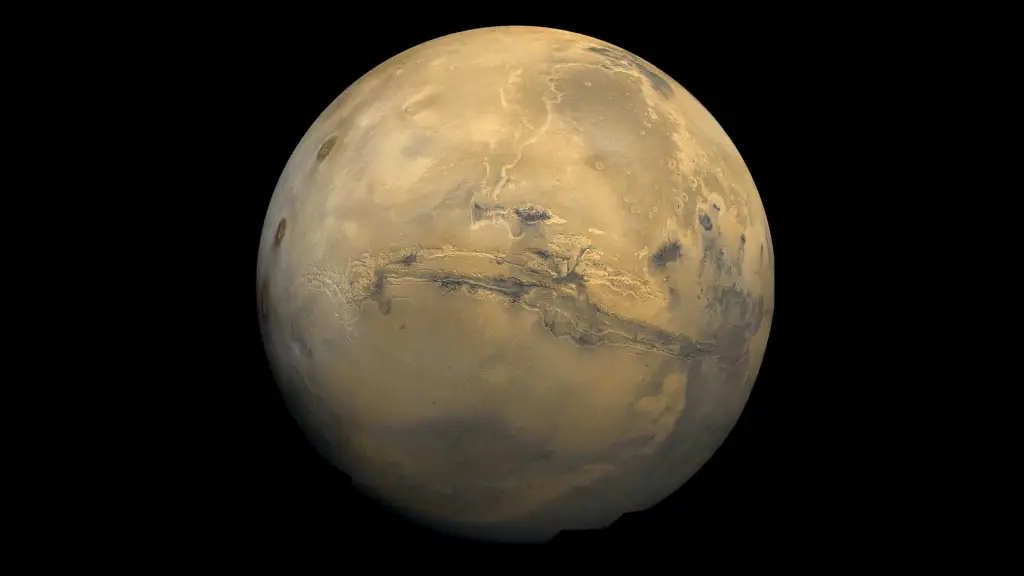
\includegraphics[width=\linewidth]{mars.png}
        \caption{Mars}
        \label{fig:mars}
    \end{subfigure}
    \vspace{0.5cm}\\
    \textbf{Outer Planets}\\
    \vspace{0.5cm}
    \begin{subfigure}{0.2\textwidth}
        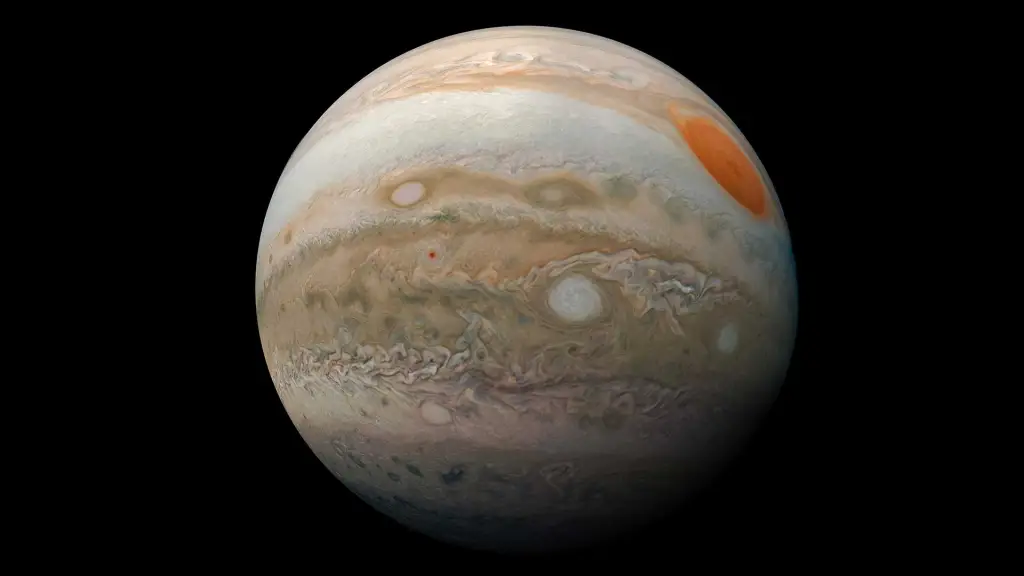
\includegraphics[width=\linewidth]{jupiter.png}
        \caption{Jupiter}
        \label{fig:jupiter}
    \end{subfigure}
    \hfill
    \begin{subfigure}{0.2\textwidth}
        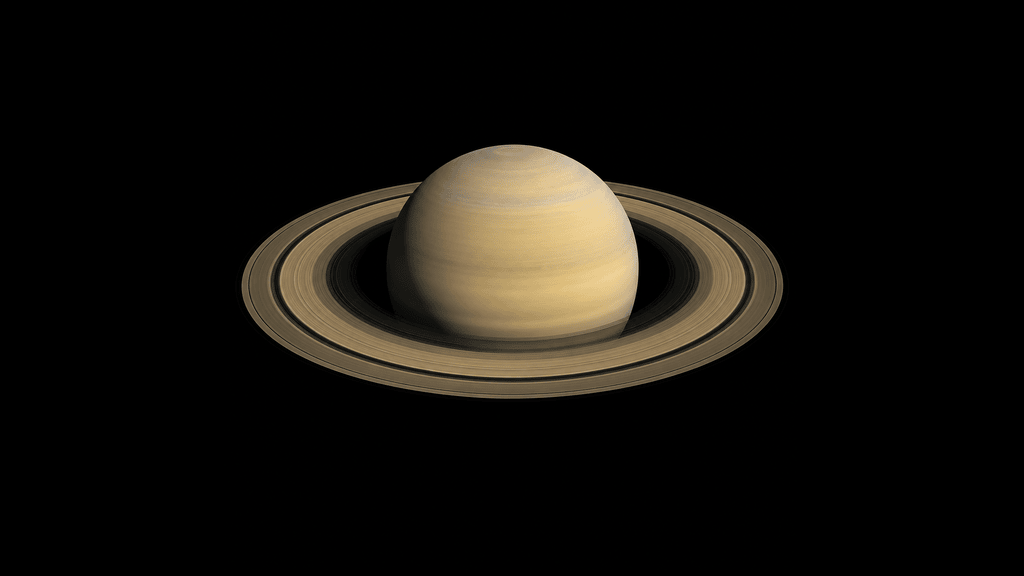
\includegraphics[width=\linewidth]{saturn.png}
        \caption{saturn}
        \label{fig:saturn}
    \end{subfigure}
    \hfill
    \begin{subfigure}{0.2\textwidth}
        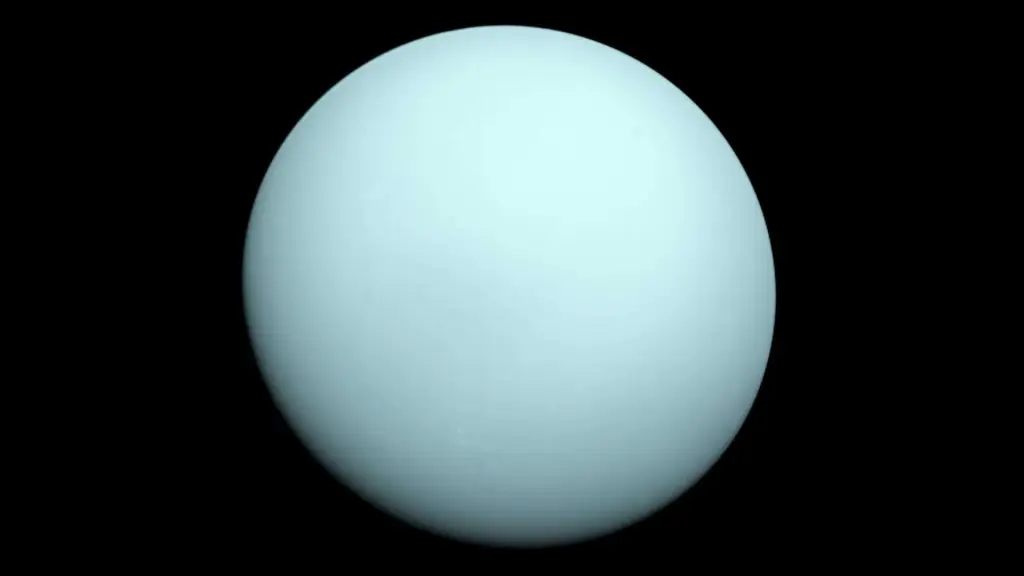
\includegraphics[width=\linewidth]{uranus.png}
        \caption{uranus}
        \label{fig:uranus}
    \end{subfigure}
    \hfill
    \begin{subfigure}{0.2\textwidth}
        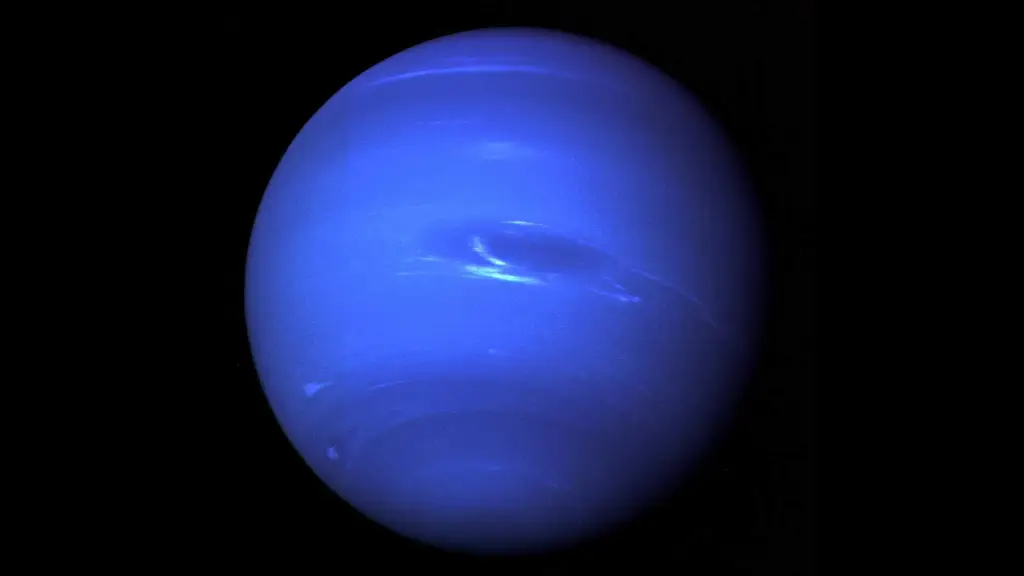
\includegraphics[width=\linewidth]{neptune.png}
        \caption{neptune}
        \label{fig:neptune}
    \end{subfigure}

    \caption{The Sun and the eight planets of the Solar System, arranged into the inner and outer planetary groups. The displayed sizes and distances are not to scale.}
    \label{fig:solar}
\end{figure}

\section{Kepler’s Laws of Planetary Motion}
Kepler’s three laws describe planetary motion \cite{nasa_kepler}.


\subsection{First Law: Elliptical Orbits}
A planetary orbit is elliptical, with the Sun at one focus:
\be
\frac{x^2}{a^2} + \frac{y^2}{b^2} =  1, \quad a \ge b > 0.
\ee
Here $a$ and $b$ are the semi-axes.

For focal distance $c$,
\begin{align}
    c^2 &= a^2 - b^2 \notag \\
    e &= \frac{c}{a}\\
\end{align}
Here $e$ is the eccentricity.

In polar form,
\be
r(\theta) = \frac{a(1-e^2)}{1+e\cos\theta}
\ee


\subsection{Second Law: Equal Areas in Equal Times}
Equal times sweep equal areas:
\be
\Delta t_1 = \Delta t_2 \implies \Delta A_1 = \Delta A_2
\ee

Consequently, a planet moves
\begin{itemize}[label=$\diamond$]
    \item faster when it is closer to the Sun, and
    \item slower when it is farther from the Sun.
\end{itemize}
% $\diamond$ faster when it is closer to the Sun, and \\
% $\diamond$ slower when it is farther from the Sun.

\subsection{Third Law: Orbital Period and Distance}
For planets orbiting one star,
\be
T^2 \propto a^3
\ee
Newtonian form:
\be
T^2 = \frac{4\pi^2}{GM_{\odot}}a^3,
\ee
Here $M_{\odot}$ is the solar mass.
\subsection{An Earth–Mars Comparison}
Using Earth as reference,
\[
a_E = 1 \text{AU} \quad \quad \quad T_E = 1 \text{year}
\]
where $1 \text{ AU} \approx 1.496 \times 10^{11} \text{m}$\footnote{AU denotes the mean Earth–Sun distance} For Mars, $a_M \approx 1.524 \text{ AU}$, so
\begin{align}
\frac{T_M ^2}{T_E ^2} &= \frac{a_M^3}{a_E^3} \notag\\
   T_M &= T_E \left( \frac{a_M}{a_E}\right)^{3/2} \notag\\
    &\approx (1.524)^{3/2} \approx 1.88 \text{years} \notag
\end{align}


Thus, $T_M \approx 1.88$  years.

\section{A Relativistic Extension}
General relativity extends Kepler’s model.\footnote{Planetary corrections are small but measurable.} Einstein’s equations are
\be
G_{\mu \nu} + \Lambda g_{\mu\nu} = \frac{8\pi G}{c^4} T_{\mu\nu}
\ee
For spherical mass $M$,
\be
ds^2 = - (1-\frac{r_s}{r} )c^2 dt^2 + (1-\frac{r_s}{r} )^{-1}dr^2 \\
+ r^2 (d\theta^2 + \sin^2\theta d\phi^2), \quad r_s = \frac{2GM}{c^2}.
\ee
Free fall satisfies
\be
\frac{d^2 x^{\mu}}{d\tau^2} + \Gamma_{\alpha\beta}^{\mu} \frac{d x^{\alpha}}{d\tau} \frac{d x^{\beta}}{d\tau} = 0
\ee

Per orbit,
\be
\Delta \varphi = \frac{6\pi GM}{a(1-e^2)c^2}
\ee
\begin{proposition}[Weak-field circular orbit]
    For a circular orbit of radius $r$,
    \be
    (\frac{v}{c})^2 = \frac{GM}{rc^2} = \frac{r_s}{2r}
    \ee
    \label{prop:one}
\end{proposition}
\begin{proof}
    The circular-orbit balance $v^2/r = GM/r^2$ gives
    $v^2 = GM/r$. Divide by $c^2$ and use $r_s = 2GM/c^2$.
\end{proof}
See Proposition \ref{prop:one}.
\section{The Outer Planets}
The outer planets are Jupiter, Saturn, Uranus, and Neptune \cite{nasa_planets}. The first two
are gas giants; the last two are ice giants.
Table \ref{tab:one} uses scientific and relativistic notation.\footnote{Values are rounded for typesetting practice.}

\begin{table}[h]
    \centering
    \begin{tabular}{|c|c|c|c|c|}
        \hline
        \multirow{2}{*}{Planet} & \multicolumn{2}{|c|}{Orbital parameters} & \multicolumn{2}{|c|}{Relativistic notation} \\
        \cline{2-5}
         & $a$ (AU) & $e$ & $\varepsilon$ & $\beta=\sqrt{\varepsilon}$ \\
         \hline
         Jupiter & $5.204$ & $4.89 \times 10^{-2}$ & $1.90 \times 10^{-9}$ & $4.36 \times 10^{-5}$ \\
         \hline
         Saturn & $9.583$ & $5.65 \times 10^{-2}$ & $1.03 \times 10^{-9}$ & $3.21 \times 10^{-5}$ \\
         \hline
        Uranus & $19.191$ & $4.72 \times 10^{-2}$ & $5.14 \times 10^{-10}$ & $2.27 \times 10^{-5}$ \\
        \hline
        Neptune & $30.070$ & $8.6 \times 10^{-3}$ & $3.28 \times 10^{-10}$ & $1.81 \times 10^{-5}$\\
        \cline{1-5}
    \end{tabular}
    \caption{ Orbital and relativistic parameters of the outer planets}
    \label{tab:one}
\end{table}

Table \ref{tab:one} compares the four giant planets.
\printbibliography
\end{document}
